\section{tasks::interlacedwavecal Class Reference}
\label{classtasks_1_1interlacedwavecal}\index{tasks::interlacedwavecal@{tasks::interlacedwavecal}}
Inheritance diagram for tasks::interlacedwavecal::\begin{figure}[H]
\begin{center}
\leavevmode
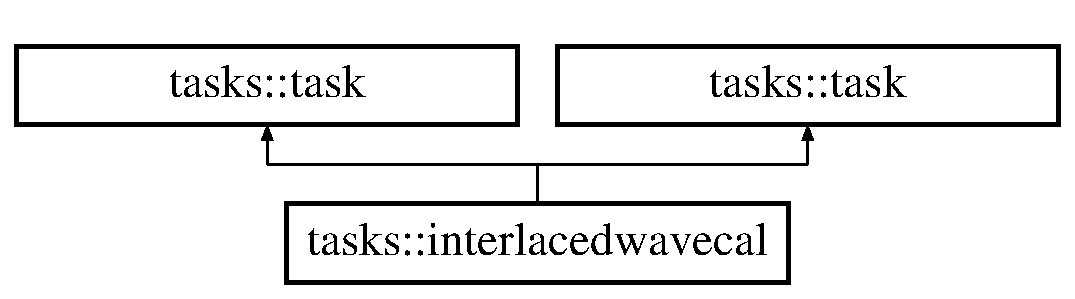
\includegraphics[height=2cm]{classtasks_1_1interlacedwavecal}
\end{center}
\end{figure}
\subsection*{Public Member Functions}
\begin{CompactItemize}
\item 
def \textbf{run}\label{classtasks_1_1interlacedwavecal_655d3dfa01de46e8e87697a3c15b2a1b}

\item 
def \textbf{run}\label{classtasks_1_1interlacedwavecal_655d3dfa01de46e8e87697a3c15b2a1b}

\end{CompactItemize}
\subsection*{Static Public Attributes}
\begin{CompactItemize}
\item 
string \textbf{name} = '{\bfinterlacedwavecal}'\label{classtasks_1_1interlacedwavecal_251335a48c77ae2f64e3a15a97a3b538}

\item 
string \textbf{button\-Text} = 'Find interlaced wavel. sol.'\label{classtasks_1_1interlacedwavecal_1523b5ec48279a6d7b0d2717d502df92}

\item 
list \textbf{prereq} = ['{\bffindinterlacedord}']\label{classtasks_1_1interlacedwavecal_7701eea0fc0e158326ad333d832fbbc7}

\item 
int \textbf{inthread} = 0\label{classtasks_1_1interlacedwavecal_7575699f1d492ad610df24a9c07cae45}

\end{CompactItemize}


\subsection{Detailed Description}


\footnotesize\begin{verbatim}Interactively determine a 2-dimensional wavelength definition from a
   well-exposed interlaced wavelength definition frame, normally an ThAr frame.
\end{verbatim}
\normalsize
 



The documentation for this class was generated from the following files:\begin{CompactItemize}
\item 
old/PANICtool-1.0/tasks.py\item 
old/tasks.py\end{CompactItemize}
